\pdfoutput=1

\documentclass{l4proj}

%
% put any packages here
%
\usepackage{color}
\usepackage{gensymb}
\usepackage{colortbl} 
\usepackage{xcolor} 
\usepackage{xfrac}
\usepackage{etoolbox}

\makeatletter
\patchcmd{\@classz}
  {\CT@row@color}
  {\oldCT@column@color}
  {}
  {}
\patchcmd{\@classz}
  {\CT@column@color}
  {\CT@row@color}
  {}
  {}
\patchcmd{\@classz}
  {\oldCT@column@color}
  {\CT@column@color}
  {}
  {}
\makeatother


\graphicspath{ {images/} }

\begin{document}
\title{ChessBaxter}
\author{Lorenzo Betto}
\date{March 21, 2017}
\maketitle

\begin{abstract}
The purpose of this project is to develop computer vision modules that allow Baxter the robot to understand the state of the chessboard and be able to inform on the next move. Since object recognition is an especially challenging problem for small objects like chess pieces, what seemed more logical was to follow the trial and error method for finding the most suitable classification model. Several computer vision and machine learning techniques were used, each giving different comparable results that helped deciding on their suitability for this particular context. 

When it came to carrying out piece recognition to detect the state of the board, machine learning was not the only field that this project explored. When the tests with machine learning classification models were not giving the expected results, the cutting-edge field of Deep Learning was also tried out and as it turns out, it performs much better than other techniques surveyed in this project. With Deep Learning it is in fact possible to perform image classification using a pre-trained classifier that is re-trained to be able to classify new objects. The final results show that deep learning is a much powerful tool for image classification and that with as little as 663 training images for six classes, it can reach more than 90\% accuracy.



\end{abstract}

\educationalconsent
%
%NOTE: if you include the educationalconsent (above) and your project is graded an A then
%      it may be entered in the CS Hall of Fame
%
\pagebreak
\section*{Acknowledgements}

I would like to thank Dr. Gerardo Arag\'on-Camarasa for the immense support he has provided throughout this entire project, going the extra mile by always being available when I needed support and explaining difficult concepts when I was not familiar with them. The achievements of this project could have never been possible without his extremely precious help and expertise.


\tableofcontents
\listoffigures
\listoftables
%==============================================================================

\chapter{Introduction}
\pagenumbering{arabic}


\section{Context}
The School of Computing Science of the University of Glasgow owns a low-cost robot called Baxter which has two arms equipped with two grippers that it can use to grab small objects. The robot has been used for several student projects and demonstrations, which include drawing a person's face on a surface using paint (Figure \ref{Baxter_drawing}) or developing the robot's ability to mimic someone's arms movements (Figure \ref{Baxter_mimicking}). These are just some of the applications that Baxter can be used for and another use would be in board games. The aim of this project is to enable Baxter to play chess like a human player would.


\vspace{10mm}
\begin{figure}[h!]
\centering
\includegraphics[height=7.87cm,width=14cm]{draw.png}
\caption{Baxter drawing someone's face \cite{Drawing}}
\label{Baxter_drawing}
\end{figure}


\vspace{25mm}
\begin{figure}[h!]
\centering
\includegraphics[height=7.87cm,width=14cm]{mimic.png} 
\vspace{2mm}
\caption{Baxter mimicking a person's arms movements \cite{Mimicking}}
\label{Baxter_mimicking}
\end{figure}



The robot was designed to perform monotonous and possibly dangerous tasks within the context of manufacturing and automation. In fact, the manufacturer's idea was to give companies a new cost-effective option for high mix, low-volume production jobs \cite{RethinkRobotics}. High-Mix Low-Volume is a manufacturing environment where the products being made vary in application, lot size and production process. High-Mix Low-Volume facilities have the ability to very quickly change over product requirements and convert assembly lines \cite{HighMixLowVolume}. Figure \ref{Baxter_working} shows Baxter in such an environment.

In the context of board games, moving pieces of a chessboard requires very little movement and effort. However, precision is necessary when it comes to dealing with small objects like chess pieces. Since Baxter is a robot that was created to deal with this kind of situations, it can then be considered compatible for such task.

\vspace{10mm}
\begin{figure}[h!]
\centering
\includegraphics[height=7.87cm,width=14cm]{baxter_working.jpg}
\caption{Baxter working in a factory \cite{RethinkRobotics}}
\label{Baxter_working}
\end{figure}


\section{Aims and Objectives}
The main idea is to make it possible for the Baxter robot to play chess against a human. The project described in this document though has the objective to detect the state of the chessboard (that is sitting on a table in front of Baxter) and output the next move that Baxter will have to execute. Consequently, this project is the beginning of the main project, i.e. make Baxter be able to play an entire chess game, and the goal is to implement a working solution that would allow Baxter to "see" the chessboard, understand it and elaborate a winning strategy. Once the project has been completed, the current intention is to show it at the Open Days helping the School of Computing Science inspire possible future students.

To the eyes of the user (a human player), Baxter should be an excellent chess player that behaves as much as possible like a friendly and competitive opponent. The idea includes creating a sense of rivalry between the user and the robot, which will enhance the user experience and make the games feel like they are played by two humans.


\section{Achievements}

The following achievements were accomplished throughout this project: 

\begin{itemize}
	\item During the design and the implementation phase of the project (Chapter \ref{DesAndImpl}) the chessboard was detected from an image and the coordinates of its outer corners were extracted. After a few tests trying what related papers demonstrated, SIFT descriptors were chosen for being scale and rotation invariant. They allowed for feature matching and the final detection of the chessboard. 
	
	The major achievement at this stage though was demonstrating that Deep Learning outperforms old machine learning techniques in image classification. After trying out different classification models combined with different feature extraction algorithms and after getting very poor results on simple tests, the initial plan changed. Deep neural networks managed to do what other techniques struggled with and the results looked promising.
	
	Finally, a chess engine was interfaced with the rest of the algorithm. After receiving the state of the chessboard as input, it outputs the best move that Baxter should execute.
	
	\item  Chapter \ref{Evaluation} outlines the performance of the system. The chessboard detection is firstly tested, followed by the algorithm for the detection of the chessboard which includes three deep neural network classifiers: the first one detects if a square contains a piece or if it is empty, the second one detects the chess piece and the third one detects its colour. The performance of the three classifiers are compared over a set of tests that helped understand where the system can improve.
	
\end{itemize}


\chapter{Literature Review}


\section{Computer Vision}

Computer vision is a field related with the way computers extract useful and meaningful information out of digital images and videos. It is concerned with the automatic extraction, analysis and understanding of useful information from a single image or a sequence of images \cite{CVBMVA}. Its ultimate goal is to use computers to emulate human vision, including learning and being able to make inferences and take actions based on visual inputs. This is why Computer Vision is considered a branch of Artificial Intelligence, whose objective is to emulate human intelligence \cite{DIP}.

When talking about computer vision, it is important to mention the areas of digital image processing and machine learning, with which computer vision overlaps considerably. They are both fundamental to reach the desired output in an application that requires the computer to see something in a scene.

Digital image processing is the field related to the manipulation of digital images in order to make them better for a specific purpose. Often this means that particular features or patterns in an image have to be highlighted so that the output image can easily be manipulated depending on the application that one is dealing with \cite{DIPTartu}. For example in Figure \ref{Camera_tracking}, a frame from a video captured by a camera is modified in order to highlight moving objects and the paths that they are following. 

On the other hand, machine learning uses several mathematical and statistical techniques to perform pattern recognition. The main entity in machine learning is the classifier, whose objective is to classify some input based on what it has seen before. The input can be any type of data and the output will be some description of that data that has similarities with other known data. Generally speaking, this requires an initial stage called training, where labeled data is fed to the classifier and the machine learning model will perform pattern recognition to match data belonging to the same class. When new data comes in, a prediction will be made based on what the classifier has learned.  Machine Learning is thus defined as the field concerned about learning from training data and applying the acquired knowledge to new, unseen data.

The combination of these three areas makes it possible to extract relevant and succinct information that machines can understand and use in order to achieve their goals. The chess pieces classification and the chessboard detection computed in this project were based on these paradigms. Feature extraction algorithms perform image manipulation with the intent of extracting particular features that can represent a class of objects. The better and more suitable these algorithms, the easier it is to identify specific objects by training a classifier on these features.

\vspace{10mm}
\begin{figure}[h!]
\centering
\includegraphics[height=11cm,width=7.7cm]{computer_vision.png}
\caption{A camera tracking the people walking past it \cite{ObjectTracking}.}
\label{Camera_tracking}
\end{figure}

\subsection{Deep Learning} \label{InceptionLabel}

Deep learning is a branch of Machine learning that tries to emulate the way our brain works to make decisions: using neural networks. The basic unit in neural networks is the neuron, which takes some input, each with a particular associated weight, computes a function and returns an output. When neurons are stacked up together and are divided in layers, they form neural networks. Each neuron receives an input and produces an output that will be fed to another neuron. In the feed-forward model of neural networks nodes in the lower layers feed neurons in the higher layers, whereas in recursive neural networks nodes in higher layers can feed nodes in lower layers too. The nodes in the final layer produce the final output \cite{DeepLearning}.

\begin{figure}[h!]
\centering
\includegraphics[height=5.8cm,width=14cm]{neural_network2.png}
\caption{An example of a 3-layer neural network.}
\label{Neural_network}
\end{figure}

In 2014 Google developed and distributed Tensorflow, a machine learning library especially useful when working with neural networks. TensorFlow was developed by researchers and engineers working on the Google Brain Team within Google's Machine Intelligence research organization for the purposes of conducting machine learning and deep neural networks research, but the system is general enough to be applicable in a wide variety of other domains as well \cite{TensorFlow}. Tensorflow uses a pre-trained classifier called Inception V3 that was trained with the data present on ImageNet in 2012 (1.2 million images for a total training time of two weeks with an 8-GPU fast desktop computer \cite{Inception}) and was implemented for the ImageNet Large Visual Recognition Challenge. At its basic state, it can differentiate between 1000 classes, including for example dishwashers and dalmatians \cite{TensorFlowForPoets}. Figure \ref{DeepClassificationPicture} shows four examples of the performance of Inception.

\begin{figure}[h!]
\centering
\includegraphics[scale=0.4]{classification.png}
\caption{Inception example of classifications on four images \cite{TensorFlowClassification}.}
\label{DeepClassificationPicture}
\end{figure}

According to TensorFlow's tutorial \cite{Retraining} the idea is to use transfer learning, which means adding a new layer on top of what the classifier has already learned. This last layer before the final output layer is called Bottleneck and it has been trained to output a set of values that is good enough for the classifier to use to distinguish between all the classes it was meant to recognise. As stated by TensorFlow's tutorial, the reason the final layer retraining can work on new classes is that the information needed to distinguish between the classes in ImageNet is often also useful to distinguish between new objects. In order to speed up the retraining process, since every image is reused multiple times each bottleneck is saved on disk so it does not have to be calculated again whenever a new retraining is needed. Following from TensorFlow's tutorial, once the bottlenecks have been saved on disk, the actual training of the top layer of the network begins. The algorithm outputs three values for each step: training accuracy, validation accuracy and cross entropy. The training accuracy shows how many images that were already used for training were labeled correctly. The validation accuracy on the other hand uses a random set of pictures from the part of the training data that has not been used yet. If the train accuracy is high but the validation accuracy remains low, the classifier is remembering features in the training images that are not meaningful and do not describe the objects that want to be classified. The final output of each step is the cross entropy value, which is a loss function that shows how well the training is going. The smaller the cross entropy, the better \cite{Retraining}.

Finally, TensorFlow's tutorial states that the default value of training steps is four-thousand and that at each step the algorithm chooses 10 random images from the training set and feeds them into the final layer to get predictions. A comparison against the actual labels is used to update the final layer's weights through a back-propagation process. At the end of the retraining, a final test accuracy evaluation is run on a set of images that were not used for the retraining and this value shows a prediction on how well the model will perform \cite{Retraining}.

\subsection{OpenCV}

OpenCV is an open-source software library that supports computer vision applications. It is released under a BSD (Berkeley Software Distribution) license and hence it is free for both academic and commercial use. It supports Windows, Linux, Mac OS, iOS and Android \cite{OpenCV}. It is widely used all around the world and its community is made up of about 47 thousand people. Many OpenCV's classes and functions will be used throughout this project.




\section{Robotics}

Robotics is a branch of engineering that involves the conception, design, manufacture and operation of robots \cite{WhatIsRobotics}. It is directly related to the fields of computing science, artificial intelligence and electronics. In 1941 Isaac Asimov, a science fiction writer, writes the short story 'Liar!' in which he describes the Three Laws of Robotics and is often credited for being the first person to use the term robotics \cite{RoboticsWordCoined}. The renowned Three Laws of Robotics are:

\begin{enumerate}
	\item A robot may not injure a human being or, through inaction, allow a human being to come to harm.
	\item A robot must obey any orders given to it by human beings, except where such orders would conflict with the First Law.
	\item A robot must protect its own existence as long as such protection does not conflict with the First or Second Law \cite{ThreeLaws}.
\end{enumerate}

As described in Subsection \ref{Baxter}, the robot used in this project is safe to use and not dangerous to humans. Thanks to software like RViz it is possible to define where the objects and obstacles close to the robots are, avoiding collisions using motion planning (as shown in Figure \ref{RViz}). Baxter therefore complies with the Three Laws of Robotics.

\begin{figure}[h!]
\centering
\includegraphics[scale=0.53]{RViz.png}
\caption{RViz motion planning avoiding an obstacle \cite{RViz}.}
\label{RViz}
\end{figure}
\vspace{100mm}

\subsection{Baxter} \label{Baxter}

Baxter is a dual-arm low-cost humanoid and anthropomorphic robot that features cameras, joint sensors and an easy-to-learn software API based on the Robot Operating System (ROS). It is safe to use and can interact with people as its movements are elastic and not dangerous to humans. It was designed by Rethink Robotics mainly for industrial types of work but thanks to its affordability it is widely used for academic purposes as well. Baxter was manufactured in such a way that makes it suitable for continuous operations and it can run 24/7 for extended periods of time without the risk of damaging the hardware of the robot. It has state-of-the-art sensing technologies, including force, position, torque sensing and control at every joint \cite{BaxterSpecs}.
It weighs about 75kg and when it sits on the adjustable pedestal, its height ranges between 5'10" and 6'3". It is equipped, among other things, with three cameras: one on its head and two on its arms. The cameras' effective resolution is 640 x 400 pixels \cite{BaxterPhysicSpecs}. Baxter uses its two seven degree-of-freedom arms, equipped with grippers, to grab and move objects. Figure \ref{Baxter_joint_names} shows Baxter's joints that allow for smooth movements.

Baxter was not directly used for this part of the project but every design decision had to consider its characteristics and abilities. The chessboard, for example, could not be too small otherwise it would not allow for much margin of error. Another important decision influenced by Baxter's specifications was the use and the positioning of an outside camera (the Kinect). Section \ref{Discussion} explains this further.

\vspace{10mm}
\begin{figure}[h!]
\centering
\includegraphics[scale=0.8]{baxter_joint_names.png}
\caption{Baxter's joint names \cite{ArmSpecs}.}
\label{Baxter_joint_names}
\end{figure}

\vspace{10mm}

\subsection{ROS}

The Robot Operating System (ROS), as the name itself suggests, is an operating system for robots. It provides a set of open source software libraries and tools that help build robot applications. It was developed in 2006 by Willow Garage, a Californian private company that describes itself as a research laboratory and technology incubator for personal robotics, focused on research more than on profits and that has maintained close links with Stanford University. ROS is language-independent and it currently provides three main libraries to program in Python, Lisp or C++ \cite{ROS}.

ROS became popular thanks to its philosophical goals, which can be summarized by:
\begin{itemize}
	\item Peer-to-peer, which enables each robot's component to dialogue with any other component using a lookup system (service) called master.
	\item Multi-language: due to the fact that the ROS specification works at the messaging layer, peers can communicate using XML-RPC, which exists in many languages.
	\item Tools-based: ROS uses a large number of small tools that bring in robustness and flexibility. Any ROS command is an executable. If an executable does not work the system will not be affected. This makes ROS more robust and flexible than a centralised runtime environment.
	\item Thin, to allow for reusability. In fact, developers are encouraged to write standalone libraries that have no dependencies on ROS.
	\item Free and open source \cite{ROS}.
\end{itemize}

The basic element in a ROS system is a node. Nodes communicate using messages which are sent through topics via a publisher/subscriber model. The publisher node sends data on a specific topic and every subscriber node will receive that data. There can be multiple concurrent publishers and subscribers for any single topic, and a single node may publish and/or subscribe to multiple topics. Though to simplify synchronous transactions ROS uses the so called service, defined by a name, a request message and a response message. Unlike topics, there can only be one node advertising a service with a specific name \cite{ROSPaper}.

In the context of this project, ROS was used to have a publisher node providing a video stream from the Kinect as well as for a subscriber, which captures a frame from the video and saves it in a folder. The Kinect points at the chessboard while the publisher streams the video and every frame captured by the subscriber represents the state of the chessboard at a particular time. Another version of the system could publish the image directly on the topic and discard it once it has been analysed.

\section{Chess}

The origin of the game of chess is unknown but the most accepted theory is that it was invented in India around 600 A.D. A century later it was adopted in Persia, who introduced it to the Arab culture and who are consequently responsible for its later introduction into other cultures \cite{ChessOrigins}.

In 1968 one of world's best chess players, David Levy, made a bet that by 1978 no computer could beat him in a series of games. He won the bet, but he stated that he could see what was coming \cite{LevyBet}. Computers were getting better and better and in fact in 1997 a computer - IBM's Deep Blue - beat under tournament conditions the best chess player in the world for the first time in the history of this game \cite{DeepBlue}.

Nowadays there are many chess engines that could easily beat the world's best players. The most famous are Stockfish, Houdini and Komodo. Stockfish is an open-source chess engine while Houdini and Komodo are commercial engines. The Stockfish engine was developed by Tord Romstad, Marco Costalba, and Joona Kiiski. It is now being developed and maintained by the Stockfish community \cite{StockfishHP}. At the time of writing Stockfish tops the list of the best chess engines with an ELO that equals to 3392 \cite{EngineTable}. ELO is the rating system used in the world of chess to refer to how strong a player is. The best human player at the time of writing is Magnus Carlsen with an ELO rating of 2838 \cite{BestPlayers}.

The chess engine will be used in the project to allow Baxter to “think” like a professional player: it will be Baxter's intelligence.

\section{Prior Work}

Similar work was developed by other researchers but they all somehow differ from this project. The most similar project was developed at the University of Auckland, New Zealand, where Baxter was used to play chess against a human or against itself \cite{SimilarProject}. The main difference with this project is that the chessboard detection was made by simply assuming that the game started with each piece in its default position and then every square is repeatedly checked for a change of state (occupied or unoccupied by a piece). The state of a square was checked by calculating the average intensity of the square and comparing it to a hard-coded threshold. For example then, if two squares changed in state, it meant that one piece moved from square A, whose state changes from occupied to unoccupied, to square B, that had an opposite change of state. Consequently Baxter could play chess in a pure robotic way, without having any kind of interaction with the user apart from displaying a sad/happy face at the end of the game. This project should give Baxter the ability to interact more with its opponent, for example by expressing anger in case the human player tries to cheat switching two pieces to allow him a better position in the game. 

Other related works focused on chess and pieces detection using different types of cameras in different positions. One of them aimed at recording players' games for future analysis using a MacBook Pro on the side of the chessboard, with the screen more or less perpendicular to the table's surface \cite{MacProject}. To detect the chessboard they would take a picture of the chessboard without pieces on it and they would calculate the coordinates of the chessboard. Each square was then checked with heatmaps to detect the piece sitting on it. The main problem in this case was that some pieces covered others behind them and moves parallel to the camera were therefore not always well detected. Another project used a camera positioned about 50cm above the chessboard \cite{PerpendicularCameraProject}. This worked well: 162 moves of all 164 moves within three games were successfully detected by the system. The problem with the two remaining moves was that the pieces' colour was too similar to the colour of the board, making them indistinguishable. That specific position of the camera though does not seem compatible with Baxter as the chances that it would hit it would increase drastically. Finally, a project that aimed at reconstructing a chess game from a video was a good source of information to start thinking about what needed to be done throughout the project in order to detect the state of the chessboard \cite{SimilarProject2}. Their algorithm was similar to the final one used for Baxter: extraction of static pictures, detection of the board and figure recognition. 

\section{Discussion} \label{Discussion}

To achieve this project's goal the following steps will be followed. First of all the robot has to be able to recognise the chessboard and its pieces at any time. The camera had to be positioned in such a way that it would be possible for Baxter to make a move without hitting it and avoiding the camera's wire too. With this prerequisite, a 90$^{\circ}$ angle with respect to the chessboard would not be a suitable position for the camera. However, the chessboard, its squares and the pieces had to be easily distinguishable and if the camera's angle with respect to the chessboard was too close 0$^{\circ}$, some chess pieces could easily hide other pieces behind them. Consequently the camera's angle which was more suitable was about 45$^{\circ}$. Although Baxter is equipped with cameras, these do not provide good quality pictures and therefore a Kinect 2 will be used to allow better images. Kinect is Microsoft's motion sensor add-on for the Xbox 360 gaming console and even though it was developed for playing games, the technology has been applied to real-world applications \cite{Kinect}. In the final product of the main project - i.e. when Baxter plays chess - a picture will be taken as soon as the previous one has been analysed. These pictures will be processed and relevant information will be extracted out of them, i.e. the state of the board will be detected. Baxter will then check whether it is its turn because the opponent has made a move or if it still has to wait. In case Baxter has waited too long, it will pressure the opponent to make a move by, for example, agitating its arms slightly. If something has changed between two consecutive states (the opponent has made a move), Baxter will check the legality of that move and will react accordingly. Specifically, Baxter will follow these rules (assume that Baxter plays black):


\begin{itemize}


	\item If there is no difference between previous and last picture, it means there is no change in the state of the board.
	
	\item If it's the whites turn and a white piece was moved, check that the piece was moved legally. If it's not, Baxter gets angry.

	\item If it's the whites turn and a black piece disappeared, check the following picture to check if the opponent has cheated or if he/she is taking a piece(the opponent might have taken the black piece off the board before moving the white piece to take it). If no white piece has moved to the taken black piece, Baxter gets angry.

	\item If two squares have changed state or the piece that sits on them, check if castling happened and if it was allowed or if a piece was taken.

	\item If more than two pieces have changed position between two consecutive pictures, Baxter gets angry.

	\item If one more piece is introduced on the board, Baxter gets angry.


\end{itemize}

As previously described, the main differences between this project and any other previous project are the way the state of the chessboard is detected and the interaction between Baxter and the human player. It is indeed this type of interaction that creates a sense of competition between the two players and that makes the game go beyond the simple and flat chess game.


\chapter{Design and Implementation} \label{DesAndImpl}

This chapter describes the design and techniques used and developed for this project, what was tested, what worked, what did not and what changed compared to the initial plan. It compares the different mathematical and statistical models as well as the methods that were used throughout the various attempts at accomplishing each of the project's objectives. It also describes the results obtained as well as the final choice of model (where one was required) for each step.

The plan that was followed in order to achieve the goal of this project included the following main points:


\begin{enumerate}

	\item Write a script that would allow to easily and smoothly take pictures with the Kinect, storing them in a specific folder that will be accessed later on.


	\item Chessboard detection. The chessboard has to be located within an image taken by the Kinect, saving its corners' coordinates.


	\item Chess piece classification. The system has to return a prediction for an image that contains a chess piece, indicating what piece it thinks the picture contains - either rook, knight, bishop, queen, king, pawn or empty square.

	\item State of the chessboard detection.

	\item The chess engine receives the state of the board and returns the suggested next move.

\end{enumerate}


\section{Image acquisition}

Support for the Kinect is available within ROS \cite{iai_kinect2}. The node 'kinect2\_bridge' publishes video streams of different natures on different topics, as shown in Figure \ref{Kinect2_bridge}. The topic that will be used to is 'kinect2/qhd/image\_color', which shows the standard colour video.

\begin{figure}[h!]
\centering
\includegraphics[scale=0.47]{kinect2_bridge.png}
\caption{ROS topics once 'kinect2\_bridge' has been launched.}
\label{Kinect2_bridge}
\end{figure}


ROS also provides the implementation of a node that subscribes to a topic that is currently publishing a video stream and can display it on the screen. Such a node is called 'image\_view' and it accepts a parameter to specify the name of the topic. By right-clicking on the video while it is being shown, an image frame is saved to HDD. Since a constant stream of images was needed, the best option was to write a script that would use the video published on the ROS topic to save a frame every time the previous frame was analysed.

The first Python script that was needed was then aimed at taking pictures using the Kinect. The script requires the 'kinect2\_bridge' node to be running so that it can save a frame from the video while it is being streamed. By right-clicking on the video while it is being shown, a caption is taken. Since a constant stream of images was going to be needed, the best option was to write a script that would use the video published on the ROS topic to save a frame every few seconds. Section \ref{PieceClassLabel} explains how this script was used. Figure \ref{ROSNodesRunning} shows the two aforementioned nodes running and showing a video stream from the Kinect.

\begin{figure}[h!]
\centering
\includegraphics[scale=0.26]{kinect2_bridge_roslaunch.png}
\caption{'kinect2\_bridge' and 'image\_view' running.}
\label{ROSNodesRunning}
\end{figure}

\vspace{10mm}

\section{Chessboard Detection} \label{Chessboard_Detection}

Detecting the chessboard in a picture can be done using the so-called feature matching algorithm, which extracts features from a sample image of the object we want to detect and tries to find the same features in the image where we want to detect the object. To be more detailed, the algorithm finds key points, which are particular points of an image where, for example, a change of light occurs, and each of these is converted to a descriptor, which is a vector representing the specific feature. Once enough features are matched, the object is recognised and the features can be matched and displayed like in Figure \ref{matched_features}.


The first attempt to detect the chessboard involved using a function called findChessboardCorners(), which takes as arguments an image and the number of inner corners per row and column - in case of a standard chessboard this would be (7,7). The expected result is shown in Figure \ref{findChessboardCorners}, but this function did not work with the chessboard used in this project. The problem is related to the colour of the chessboard, which is made of wood and uses two different shades of brown to represent the black and white squares, as shown in Figure \ref{MyChessboard}. Converting the image to grayscale did not help either, indicating that the function expects the colours of the chessboard to be almost pure black and pure white.


\begin{figure}[h!]
\vspace{7mm}
\centering
\includegraphics[height=7cm,width=14.5cm]{chessboard_normal_and_b&w.jpg}
\caption{The chessboard used in this project. Colour variant to the left and grayscale to the right.}
\label{MyChessboard}
\end{figure}

\begin{figure}[h!]
%\vspace{10mm}
\centering
\includegraphics[height=7cm,width=7.5cm]{findChessBoardCorners.png}
\caption{findChessboardCorners() in action \cite{FindChessboardCorners}.}
\label{findChessboardCorners}
\end{figure}


Since the above approach was not suited for the purpose of this project, a robust feature extraction technique was performed using SIFT (Scale-Invariant Feature Transform) descriptors, which are 128-dimensional vectors. As proved by David Lowe in his paper, SIFT features are invariant to image scaling and rotation, and partially invariant to change in illumination \cite{DavidLowe}, which makes them perfect for this purpose. To perform the chessboard detection, an orthogonal picture of the chessboard was taken and cropped, in order to avoid detecting key points from external sources. Once the descriptors are extracted from this picture and from the picture in which the program is trying to locate the chessboard, a matching algorithm is used to pair up the most similar features. FLANN (Fast Library for Approximate Nearest Neighbors) based matcher is the algorithm used in this case and as opposed to the Brute-Force matcher, FLANN is much faster since it does not compare each descriptor from one image with every other descriptor from the other image. Instead, it uses the nearest neighbors first and their proportional distance in order to avoid false positives.

The algorithm gave immediately the expected results: 41 key points with their corresponding descriptors were extracted as shown in Figure \ref{matched_features}

\vspace{5mm}
\begin{figure}[h!]
\centering
\includegraphics[scale=0.25]{matched_features.png}
\caption{Matched features between the two chessboard images.}
\label{matched_features}
\end{figure}

At this point, a homography of the chessboard served to make sure the object was detected precisely. Figure \ref{homography} shows that the chessboard was correctly detected and located in the image.

\vspace{5mm}
\begin{figure}[h!]
\centering
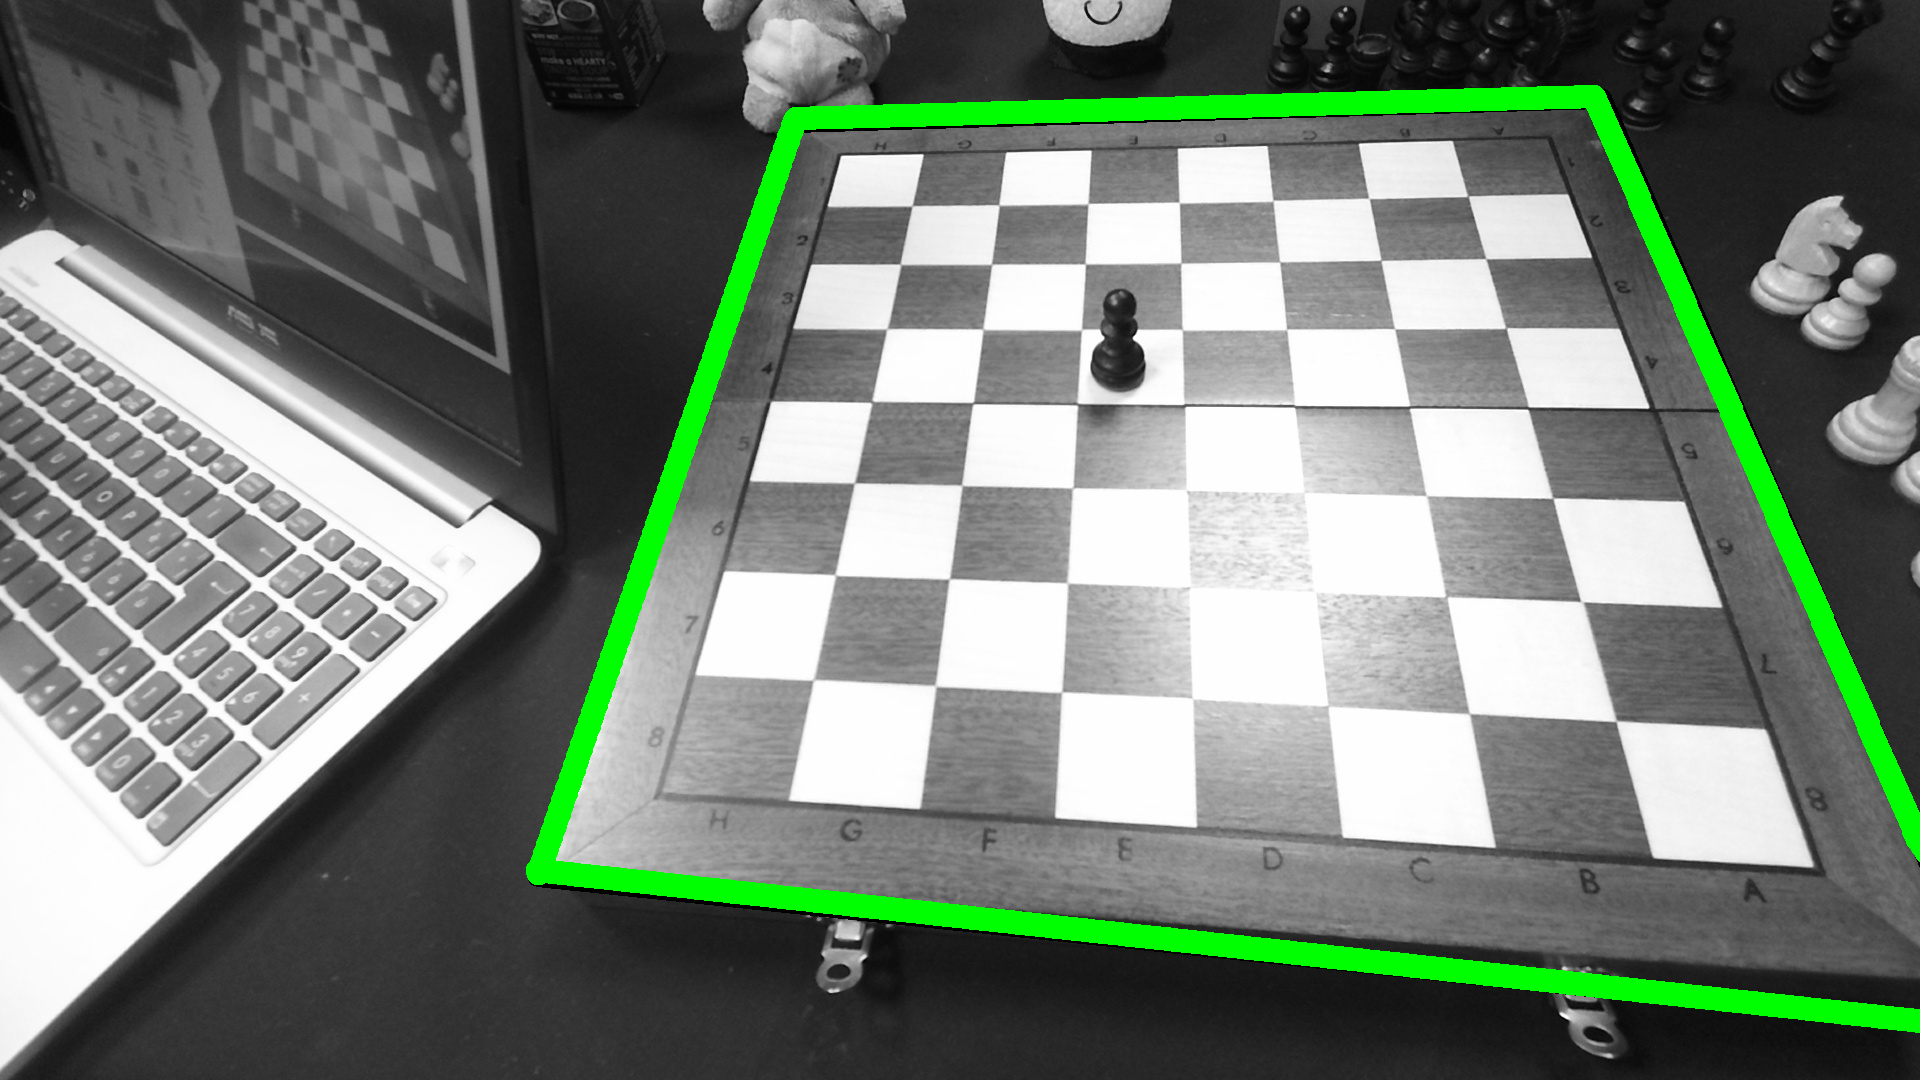
\includegraphics[scale=0.29]{homography2.png}
\caption{Chessboard homography.}
\label{homography}
\end{figure}

After the correct localisation of the object, the chessboard had to be segmented. In fact, looking ahead of what could have helped when trying to detect the pieces, saving each square's location was going to be extremely useful. Using Ubuntu's image editor GIMP, it was possible to save the (x,y) coordinates of each outer corner on the chessboard from the original orthogonal picture (Figure \ref{MyChessboard}, whichever variant). A text file now contained the 36 coordinates (9 per chessboard side, including 4 repetitions for the four actual corners) and it was used to draw lines from each corner to its orthogonally opposite one. The final output of the chessboard segmentation resulted in a more accurate visual feedback on the precision of the detection.

\vspace{5mm}
\begin{figure}[h!]
\centering
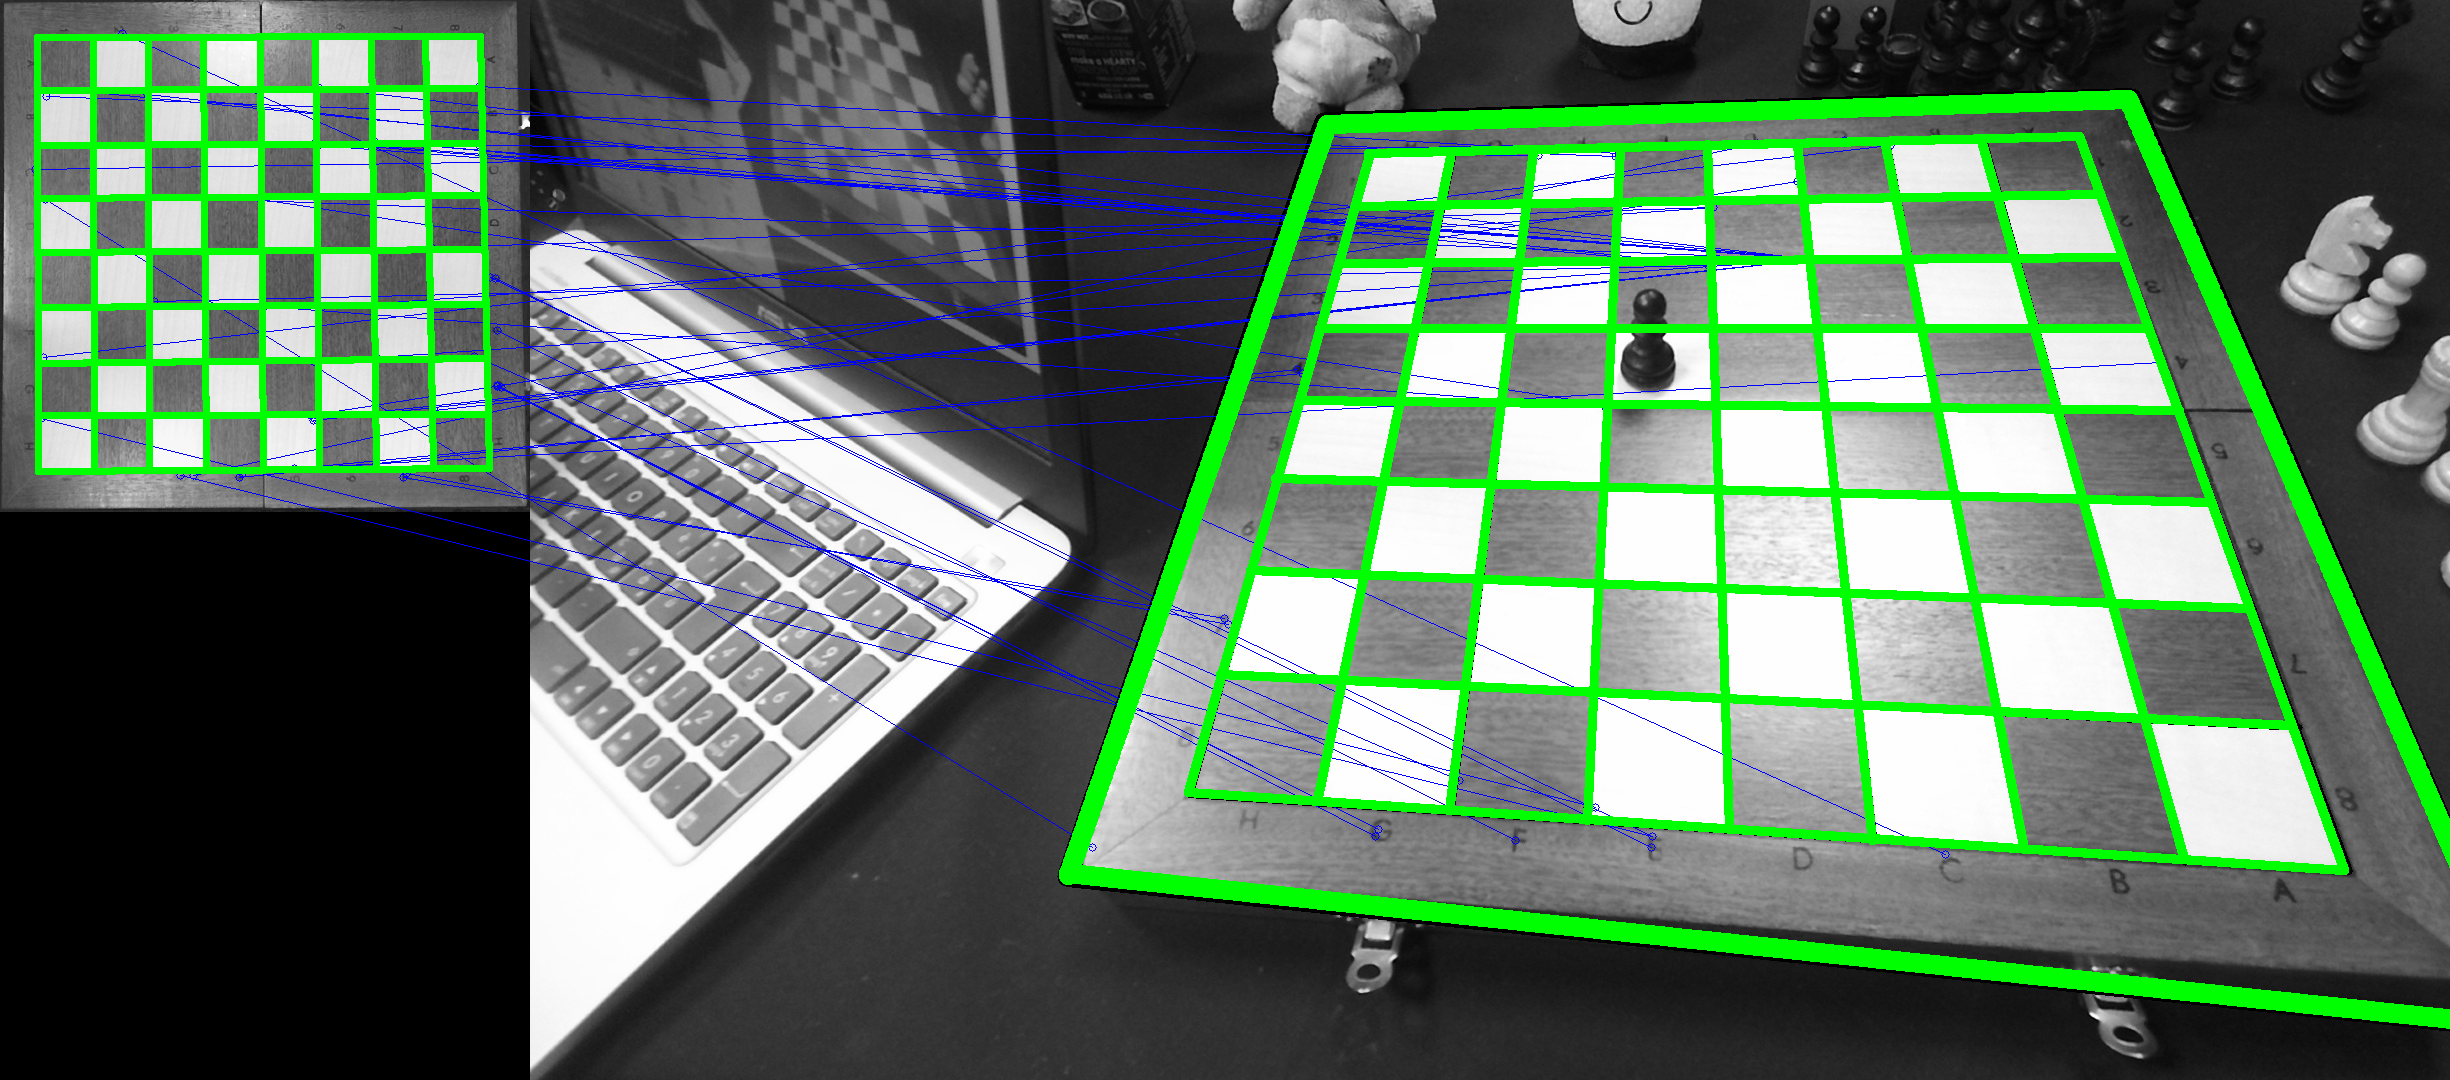
\includegraphics[scale=0.27]{homography_with_lines3.png}
\caption{Chessboard homography and segmentation.}
\label{homographyAndSegmentation}
\end{figure}

\section{Piece classification} \label{PieceClassLabel}

Training data was required in order to compute image classification to distinguish the various chess pieces. The Python script written earlier on and described in Section 3.1 served for this purpose. The pictures of the chess pieces were taken at different angles and from different distances within a certain range to allow the classifiers to generalise. Generalisation occurs when the classifier has captured the differences among the objects of different classes and the similarities among the objects of the same class.

%\vspace{10mm}
\begin{figure}[h!]
\centering
\includegraphics[scale=0.25]{king_on_table.jpeg}
\caption{An example of the pictures that were taken to build the training data, all about one meter away from the piece.}
\label{KinectPictureKing}
\end{figure}

After the first session, 480 pictures in total were taken walking around a table with the camera pointing at the piece that is sitting on it, like shown in Figure \ref{KinectPictureKing}. Following the removal of the blurry images caused by the movement of the Kinect around the table, 260 pictures were left (about 130 per colour), with an average of 43 pictures per piece (21 if considering the type of piece and its colour).  Figure \ref{BishopSetOfPictures} shows the pictures that were selected for the bishop. The pictures now needed to be cropped to remove noise and to be able to extract the features only from the chess pieces, ignoring the background and the other objects lying around. Keeping in mind that the first achievement would be to be able to detect a piece from another independently of its colour, only the pieces of one of the two colours were cropped - white was randomly picked. In case the algorithm had given satisfying results, it would have been extended to include the black pieces too. 

Each picture had a resolution of about 50x100 pixels and looked like the picture of the knight shown in Figure \ref{CroppedKnight}. Figure \ref{BishopFolderNoBG} shows the folder of the bishop's cropped pictures. Considering how the subject of the picture was the same and it was not moved between one picture and another, it is easy to see how the pictures cover a fair range of values in terms of angle and direction of the exposure to the light. 

\vspace{10mm}
\begin{figure}[h!]
\centering
\includegraphics[scale=1.5]{white_knight7.png}
\caption{A perfectly cropped picture of the knight (NB: The size of this picture was doubled to make it more visible.}
\label{CroppedKnight}
\end{figure}


\vspace{20mm}
After creating the database of images, the idea was to try out different classification models and eventually use the one that fitted the best. Another variable of the system was the type of feature descriptors. At this stage the methodology that was followed was 'trial and error'. Many in fact are both the types of feature descriptors as well as the classification models available and supported with open-source libraries, which allowed for relatively fast testing.



\begin{figure}[h!]
\centering
\includegraphics[scale=0.5]{first_pictures.png}
\caption{The non-blurry photos selected to represent the bishop.}
\label{BishopSetOfPictures}
\end{figure}



\begin{figure}[h!]
\centering
\includegraphics[scale=0.40]{bishop_folder_noBG.png}
\caption{Training data for the bishop.}
\label{BishopFolderNoBG}
\end{figure}


\pagebreak
\subsection{Feature descriptors}

Each feature descriptor works in a different way and works better in a particular case. Using the libraries available online it was possible to test the following different ways to find the key points and compute their descriptors:

\begin{itemize}

	\item SIFT (Scale-Invariant Feature Transform). As described in Section 3.3, it is an algorithm that computes 128-dimensional vectors representing each key point and it is invariant to image scaling and rotation, and partially invariant to change in illumination.

	\item ORB (Oriented FAST and Rotated BRIEF). It is a good alternative to SIFT in computation cost and matching performance. ORB is basically a fusion of FAST keypoint detector and BRIEF descriptor with many modifications to enhance the performance. First it uses FAST to find keypoints and then it applies Harris corner measure to find top n points among them. It also uses image pyramids to produce multiscale-features \cite{ORB}.

	
	\item HOG (Histogram of Oriented Gradients). The distribution (histograms) of directions of gradients (oriented gradients) are used as features in this feature extraction algorithm. Gradients (x and y derivatives) of an image are useful because the magnitude of gradients is large around edges and corners (regions of abrupt intensity changes) \cite{HOG}.

	\item Single descriptor combined with image pyramids. When extracting a single descriptor from an image, only one vector will describe the entire image. By combining this algorithm with image pyramids, it is possible to emphasise special features in an image.

\end{itemize}

Each one of these algorithms was then tested using dense key points. Dense key points force the extraction of key points from an image that might not have enough key points. This is especially useful when dealing with small images like the ones from the chess pieces, but can result in not extracting the key points that truly identify an object.

\subsection{Classifiers} \label{Classifiers}

The strategy used for the classifiers is the one-vs-all, which consists in fitting one classifier per class. Every chess piece had a classifier that is trained against every other piece. Consequently, the positive class of the training data will be represented by features of the chess piece corresponding to the specific classifier, while the negative class will be made up of features from pictures of every other chess piece. There are therefore seven classifiers, one for each chess piece plus the empty square. The classification models that were tested are:

\begin{itemize}

	\item Logistic Regression. It derives from Linear Regression but predicts the probability of an outcome that can only have two values (in this case, positive or negative detection of the relative chess piece) \cite{LRDef}.

	\item Support Vector Machine. It finds the hyperplane that best differentiates two or more classes on a multi-dimensional plane. The dimension of the plane is equal to the number of features for each vector \cite{SVMDef}.

	\item KNN. Data is classified according to which class the k-nearest vectors belong to (each vector representing one data sample).The distance the KNN algorithm uses is the Euclidean distance, given by the following formula:
	
	\begin{figure}[h!]
	\centering
	\includegraphics[scale=0.15]{euclidean_formula.png}
	\label{EuclideanDistance}
	\end{figure}
	\pagebreak
	where x and y are two n-dimensional vectors. The only parameter that can be modified to tweak this type of classifier is k, which is the number of neighbours we want to count when classifying data \cite{KNN}.

	\item Colour Histograms. A histogram is a graphical representation of the value distribution of a digital image. The value distribution is a way to represent the colour appearance. Histograms are invariant to translation and they change slowly under different view angles, scales and in presence of occlusions \cite{ColourHist}.
	
\end{itemize}

\subsection{Process and Results}

Cross-validation is a standard method used in machine learning to verify how well a classifier is performing. In the basic approach, called k-fold CV, the training set is split into k smaller sets. The following procedure is followed for each of the k "folds" \cite{CrossVal}:

\begin{itemize}

	\item A model is trained using k-1 of the folds as training data.
	\item The resulting model is validated on the remaining part of the data (i.e., it is used as a test set to compute a performance measure such as accuracy). 

\end{itemize}

The performance measure reported by k-fold cross-validation is then the average of the values computed in the loop \cite{CrossVal}. The main data that will be used to compare the several methodologies used will then be mainly the result of cross-validation. Once the accuracy from the cross-validation was high enough, the classifier would be tested with a sample sliding window (a cropped image containing a chess piece - explained in Section \ref{Sliding_Window}). Furthermore, scikit-learn's 'joblib' library helped model-persistence. After training a scikit-learn model, it is desirable to have a way to persist the model for future use without having to retrain it. 'joblib' is a replacement for Python's built-in persistence model 'pickle' and it is more efficient on objects that carry large numpy arrays internally as is often the case for fitted scikit-learn estimators \cite{ModelPersistence}.

The first problem that arose was that SIFT could not detect enough descriptors for the empty square. A decision was made at this point to exclude temporarily the empty square from the classification algorithm, in order to prioritise the distinction amongst the chess pieces. The goal was to reach an accuracy of at least 0.85 before moving on to the next step.

The first classifier followed a multiclass model, which means it performed classification with more than two classes \cite{MultiClass}. It was trained with six classes, one per chess piece type, with the intent of having only one classifier and saving running time. An SVM classifier with SIFT descriptors only returned an accuracy of 0.32, indicating that this strategy was wrong and had to be changed. One-vs-all, as described in Subsection \ref{Classifiers}, was the strategy followed for every other test: each chess piece had a corresponding classifier that given a sliding window would indicate the confidence of that image containing the relative chess piece.

The second test aimed at classifying a pawn from the rest of the pieces, therefore the training data used the pawn cropped pictures for one class and every other piece for the second class. Using  ORB descriptors and an SVM classifier, the accuracy returned was equal to 0.70. When tested with unseen images of a pawn though, it would perform extremely poorly, never classifying the piece as a pawn. At this point, a series of tests involving several variables started. First of all the training images changed from having a transparent background, to a black background (which in terms of matrix representation would fill up the matrix with zeros) and eventually to including some background noise as well. Figure \ref{Images_changing} shows how the pictures changed. The number of images also increased from an average of 21 up to about 50 images per chess piece, including both black and white pieces.

\begin{figure}[h!]
\centering
\includegraphics[scale=0.5]{sequence_of_queens.png}
\caption{Three samples from the first, second and third set of queen images.}
\label{Images_changing}
\end{figure}

In regard to the feature extraction techniques, dense features were also tried out with ORB, SIFT and HOG. Due to the poor results though, they were not used again. Another change was with respect to the proportion between the number of descriptors for the positive class (the pawn) and the number of descriptors for the negative class. Since the ratio was always between 1:6 and 1:12, the number of descriptors for the negative class was reduced in such a way that the final ratio would be 1:1 and 1:2, for two different tests. Again, the results on the accuracies were around 0.80 (using different feature extractors) but when tested on pictures that the classifiers had not seen before, they would not be able to classify correctly.

The following tables refer to tests run with 33 images per chess piece, all white pieces with a black background and a few pixels of noise around the piece figure. Tables \ref{SIFTTable1} and \ref{SIFTTable2} use SIFT as feature extractor, Tables \ref{ORBTable1} and \ref{ORBTable2} use ORB and finally Tables \ref{HOGTable1} and \ref{HOGTable2} use HOG features. Furthermore, a classifier was trained to simply detect a pawn against a king in order to observe what the results were and help understand where the problem might be. These two pieces were picked for these tests because they look very different from each other.



\begin{table}[h!] \label{SIFTTable1}
	\centering
	\textbf{SIFT}
	
	\vspace{2mm}
	\begin{tabular}{|c|c|}
	\hline
	Chess Piece & N. of Descriptors  \\
	\hline
	\rowcolor{brown!45} Bishop & 1120 \\
	King & 1953 \\
	\rowcolor{brown!45} Knight & 1137 \\
	Pawn & 929 \\
	\rowcolor{brown!45} Queen & 1680 \\
	Rook & 1435 \\
	\hline
	\end{tabular}
\end{table}



\begin{table}[h!] \label{SIFTTable2}
	\centering
	\begin{tabular}{|c|c|c|c|c|} 
	\hline
	 & SVM & LR & KNN & Mean  \\
	\hline
	\rowcolor{brown!45} Cross-validation Accuracy - PawnVsTheRest & 0.89 & 0.88 & 0.89 & 0.886667 \\
	Cross-validation Accuracy - PawnVsKing & 0.68 & 0.69 & 0.75 & 0.706667\\
	\rowcolor{brown!45} Correct classification of previously seen picture of a pawn (PawnVsTheRest) & Y & N & N & 1/3 \\
	Correct classification of an unseen picture of a pawn (PawnVsTheRest) & N & N & N & 0/3 \\
	\rowcolor{brown!45} Correct classification of previously seen picture of a king (PawnVsTheRest) & Y & Y & Y & 3/3 \\
	Correct classification of an unseen picture of a king (PawnVsTheRest) & Y & Y & Y & 3/3 \\
	\hline
	\end{tabular}
	\caption{Results from SVM, LR and KNN using SIFT features.}
\end{table}

	

\begin{table}[h!] \label{ORBTable1}
	\centering
	\vspace{10mm}
	\textbf{ORB}
	
	\vspace{2mm}
	\begin{tabular}{|c|c|} 
	\hline
	Chess Piece & N. of Descriptors  \\
	\hline
	\rowcolor{brown!45} Bishop & 6649 \\
	King & 10086 \\
	\rowcolor{brown!45} Knight & 5110 \\
	Pawn & 4973 \\
	\rowcolor{brown!45} Queen & 9092 \\
	Rook & 5421 \\
	\hline
	\end{tabular}
\end{table}


\begin{table}[h!] \label{ORBTable2}
	\centering
	\begin{tabular}{|c|c|c|c|c|} 
	\hline
	 & SVM & LR & KNN & Mean  \\
	\hline
	\rowcolor{brown!45} Cross-validation Accuracy - PawnVsTheRest & 0.88 & 0.88 & 0.88 & 0.88 \\
	Cross-validation Accuracy - PawnVsKing & 0.67 & 0.67 & 0.74 & 0.693333\\
	\rowcolor{brown!45} Correct classification of previously seen picture of a pawn (PawnVsTheRest) & Y & N & N & 1/3 \\
	Correct classification of an unseen picture of a pawn (PawnVsTheRest) & N & N & N & 0/3 \\
	\rowcolor{brown!45} Correct classification of previously seen picture of a king (PawnVsTheRest) & Y & Y & Y & 3/3 \\
	Correct classification of an unseen picture of a king (PawnVsTheRest) & Y & Y & Y & 3/3 \\
	\hline
	\end{tabular}
	\caption{Results from SVM, LR and KNN using ORB features.}
\end{table}



\begin{table}[h!] \label{HOGTable1}
	\centering
	\vspace{10mm}
	\textbf{HOG}
	
	\vspace{2mm}
	\begin{tabular}{|c|c|} 
	\hline
	Chess Piece & N. of Descriptors  \\
	\hline
	\rowcolor{brown!45} Bishop & 2466 \\
	King & 2046 \\
	\rowcolor{brown!45} Knight & 3544 \\
	Pawn & 1002 \\
	\rowcolor{brown!45} Queen & 2179 \\
	Rook & 5007 \\
	\hline
	\end{tabular}
\end{table}



\begin{table}[h!] \label{HOGTable2}
	\centering
	\begin{tabular}{|c|c|c|c|c|} 
	\hline
	 & SVM & LR & KNN & Mean  \\
	\hline
	\rowcolor{brown!45} Cross-validation Accuracy - PawnVsTheRest & 0.94 & 0.94 & 0.92 & 0.933333 \\
	Cross-validation Accuracy - PawnVsKing & 0.67 & 0.75 & 0.82 & 0.7466667\\
	\rowcolor{brown!45} Correct classification of previously seen picture of a pawn (PawnVsTheRest) & N & N & N & 0/3 \\
	Correct classification of an unseen picture of a pawn (PawnVsTheRest) & N & N & N & 0/3 \\
	\rowcolor{brown!45} Correct classification of previously seen picture of a king (PawnVsTheRest) & Y & Y & Y & 3/3 \\
	Correct classification of an unseen picture of a king (PawnVsTheRest) & Y & Y & Y & 3/3 \\
	\hline
	\end{tabular}
	\caption{Results from SVM, LR and KNN using HOG features.}
\end{table}




\pagebreak
From the tables it is easy to spot how ORB, which uses 32-dimensional vector descriptors, extracted many more features than SIFT and HOG. ORB in fact extracted a total of 41331 features, 2.5 times more than HOG (16244) and 5 times more than SIFT (8254). Though ORB extracted many more features, the best accuracies were obtained with HOG, whose average across the three feature extractors is equal 0.93333.
An important result is that every unseen picture was identified as belonging to the non-pawn class and only the SVM classifier using ORB and SIFT could "remember" the previously seen picture of a pawn.
Finally, the low accuracies returned by the PawnVKing system show how the classifier was underfitting, having not enough training data.

\subsection{Conclusion of the results so far}

The results up until this point looked promising in terms of accuracy but when the classifiers were tested with images that could be the input to the final object classification module, they could not to detect the pieces. They were therefore considered not fit for purpose. A potential problem could be that the classifiers are not being able to generalise and specialise properly, which means that the classifier is not capturing the differences among the objects of different classes nor it is capturing the similarities among objects of the same class. When this happens, classes cannot be identified properly.


\section{Deep Learning and Inception} \label{DeepLearningClassification} 

Once enough tests were run and the results were not as good as expected, the strategy had to be changed. By following Google's video tutorials \cite{TensorFlowYoutubeTutorials}, it was possible to test deep neural networks without prior experience in the field. As described in subsection \ref{InceptionLabel}, Inception is a pre-trained classifier which can be retrained with new classes. By adding a new directory of subdirectories representing each class that needs to be detected and containing images of that class, it is possible to add a new layer to Inception, which will then be able to classify based on the new training data. Google's tutorials suggest using as many pictures and diversity as possible to get the best accuracy (they suggest at least 100 images per class). The training data that was going to be used for retraining Inception was the same as the one used for training the classifiers, as described in section \ref{PieceClassLabel}, which had enough pictures to get started.

The first test was to try to detect a picture of the king that could not be correctly classified with machine learning's classifiers - Figure \ref{BlackKing}. The 'Bottlenecks' directory was created in order to speed up future training time, avoiding the pictures that were already used. Among the parameters that can be defined for the training stage, TensorFlow allows to define the number of training steps. Each training step chooses 10 images at random from the training set, finds their bottlenecks from the cache, and feeds them into the final layer to get predictions. Those predictions are then compared against the actual labels to update the final layer's weights through a back-propagation process \cite{TensorFlowForPoets}. With five-hundred training steps, the training took 1 minute and 20 seconds and it returned 100\% final test accuracy. This result reflects on the performance of the system, which accurately classifies the picture of the king with 0.87 confidence. 
With the default number of training steps, which equals to four thousand, retraining took 4 minutes and 40 seconds and it returned again 100\% final test accuracy. The test on the image of the king returned an even better result: the king is detected with 0.9705 confidence. The change in confidence demonstrates how important the training steps are and it is worth waiting longer during the training stage to get better performances. Every retraining from now on will be run with the default value of training steps.

\begin{figure}[h!]
\centering
\includegraphics[scale=1]{king.jpg}
\caption{A sliding window with a king and a pawn behind it.}
\label{BlackKing}
\end{figure}

Now that this simple detection worked, the training data had to be expanded to include all the other classes as well. This time retraining Inception took 9 minutes and 31 seconds and it returned 96.8\% final test accuracy.


\section{Machine learning vs Deep Learning}

The first tests using pictures of different pieces proved how deep learning outperformed the many techniques tried with machine learning. The system will then only work with TensorFlow to compute piece classification. In terms of accuracy, TensorFlow reached an only slightly higher result, especially compared to the 0.94 accuracy got with SVM and HOG descriptors as shown in Table \ref{HOGTable2}, but when it came to classify simple sliding windows with only one piece, machine learning's techniques performed very poorly while TensorFlow could confidently classify correctly in most of the cases.

\section{Sliding Window} \label{Sliding_Window}

As mentioned in Section \ref{Chessboard_Detection}, knowing the coordinates of the chessboard corners makes it relatively easy to run a sliding window with a fair precision across the chessboard. The algorithm starts with a picture of a chessboard and the coordinates of each outer corner, as explained in Section \ref{Chessboard_Detection}. The coordinates of the inner corners are unknown but it is possible to approximate fairly precisely the length for each square's bottom side, which can be used to know the length of each step that will be taken. Figure \ref{length_of_line} shows an example of the process described below.

The point where the steps will start is defined by the x value of the left-hand side outer corner and the mean of the y values of two outer corners that sit on the same line. In Figure \ref{length_of_line} the x coordinate is given by the x coordinate of point B1 and the y coordinate is given by the mean of the y coordinates of B1 and B2. These two values work for the entire row of squares above the line that joins B1 and B2. The length of a square's bottom side can be obtained by calculating the length of the line that goes from the closest outer corner until the mid point (point A in Figure \ref{length_of_line}) and by dividing this value by 4 (the 4 squares on each half row). The length of the line is obtained by calculating the euclidean distance between two points: 

\begin{itemize}
	
	\item Point A is given by the mean of the x coordinates of the two middle outer corners defines the x coordinate of the line that divides the chessboard into two parts vertically and the mean of the y coordinates of the two opposite outer corners on the side of the chessboard.
	
	\item Point B is one of the outer corners on the side of the chessboard, on the same line as point A.
	
\end{itemize}


\begin{figure}[h!]
\centering
\includegraphics[scale=0.29]{length_of_line3.png}
\caption{The length of each square's bottom side for the first row that will be classified. The length of the first four squares on the left is normally slightly different from the length of the four squares on the right and this depends on the rotation of the chessboard.}
\label{length_of_line}
\end{figure}


This process could also use the length of the entire line but it would not be as precise. The height of the sliding window is a pre-defined value that was tweaked after some tests. It was set to 110 pixels for every row except the one at the bottom, which being closer to the camera - and therefore bigger in size - needs an extra 20 pixels to be able to include tall pieces like the king. Figures \ref{row_of_pawns} shows how the sliding window looks like for the second row (starting from the top) of Figure \ref{camera_image9}. 

\begin{figure}[h!]
\centering
\includegraphics[scale=0.24]{camera_image9.jpeg}
\caption{A picture with the chessboard at the beginning of a game.}
\label{camera_image9}
\end{figure}

\begin{figure}[h!]
\centering
\includegraphics[scale=0.55]{row_of_pawns.png}
\caption{The row of white pawns from Figure \ref{camera_image9}.}
\label{row_of_pawns}
\end{figure}

Even though the Kinect is not very well aligned with the chessboard and its position is not perpendicular to the ground, it still manages to include all of the square content. The width of each sliding window is enough to include all of the chess square. The height of the bottom of the sliding window with respect to the chessboard is very precise for the two sliding windows in the middle and fairly precise for the third and fifth. Although it lacks of precision in the four outmost images, this algorithm still provides a valid solution for a quite unlikely case like this one, with the chessboard and the Kinect not very well positioned.

\pagebreak
\vspace*{20mm}
\section{Black vs White} \label{BlackVsWhite}

Considering how effective TensorFlow seemed to be as opposed to classic machine learning classification models, the same strategy was used for colour detection. A new directory called 'black\_or\_white' including two subdirectories called 'blacks' and 'whites' was added to the training data. The pictures that populate these two subdirectories are sliding windows containing either a black or a white piece accordingly. Inception is then retrained and every time a piece is detected it is also classified for its colour. If the piece is classified as white, the letter that represents it is changed to uppercase to conform to FEN notation, which is the notation used in the world of chess to represent a particular game a time \textit{t}. Section \ref{Chess_Engine} describes further how FEN works. If the piece is classified as black, the letter stays lowercase. Figure \ref{ColourDetected} shows how some letters changed case to represent their colour.

\begin{figure}[h!]
\centering
\includegraphics[scale=0.8]{detection_colour_comparison.jpg}
\caption{The detected state of the chessboard before and after colour classification.}
\label{ColourDetected}
\end{figure}

\vspace{5mm}
This particular test for colour classification was run on the Figure \ref{camera_image9} and it returned a perfect result in terms of colour classification: it kept the letters in the two bottom rows as lowercase and it changed to uppercase every letter in the two uppermost rows, which represent the white pieces.

\vspace{10mm}
\section{Final optimization of training data} \label{FinalTrainingData}

After a few tests, it was obvious that the empty square was causing most of the mistakes. That led to the implementation of a new deep net classifier that would half the height of the sliding window and classify it as either empty or with a piece on it. Besides, in order to get better classification with TensorFlow the training data needed a further expansion. A new Python script was implemented for fast training data building. The script would take a picture as input and it would take the user input on what each square contained. First of all it would show the bottom half of the sliding window, asking if it was empty or not. If it was empty, it would save it in the empty squares folder, if it was not it would save it in the non-empty folder and would show the entire sliding window asking for the name of the piece and the colour. Depending on the result, it would save the half sliding window and the entire version into the appropriate folder, ready to be used as training data by TensorFlow. The script would follow this process for each of the sixty-four squares, creating therefore considerable training data for each chessboard picture used. Figure \ref{TrainingDataBuilder} shows the aforementioned script being run.

\begin{figure}[h!]
\centering
\includegraphics[scale=0.28]{training_data_builder.png}
\caption{The 'training\_data\_builder' script running and saving the sliding windows for future retraining.}
\label{TrainingDataBuilder}
\end{figure}

\vspace{10mm}
Retraining for the chess pieces classifier took 9 minutes and returned 97.1\% final test accuracy. Retraining for the colour classifier took 5 minutes and 30 seconds and returned 100.0\% final test accuracy. Finally, retraining for the empty square classifier took 7 minutes and 15 seconds and it returned 97.1\% final test accuracy. The final training data's shape is shown in Table \ref{FinalTrainingData}.

\begin{table}[h!] \label{FinalTrainingData}

	\begin{tabular}{|c|c|}
		\hline
		Chess Piece & N. of Images  \\
		\hline
		\rowcolor{brown!45} Bishop & 104 \\
		King & 99 \\
		\rowcolor{brown!45} Knight & 117 \\
		Pawn & 135 \\
		\rowcolor{brown!45} Queen & 107 \\
		Rook & 101 \\
		\hline
		\rowcolor{brown!45} Total &  663\\
		\hline
	\end{tabular}
	\hfill
	\begin{tabular}{|c|c|}
		\hline
		Piece Colour & N. of Images  \\
		\hline
		\rowcolor{brown!45} White & 62 \\
		Black & 64 \\
		\hline
		\rowcolor{brown!45} Total &  126\\
		\hline
	\end{tabular}
	\hfill
	\begin{tabular}{|c|c|}
		\hline
		Empty or Not & N. of Images  \\
		\hline
		\rowcolor{brown!45} Empty & 173 \\
		Non-empty & 108 \\
		\hline
		\rowcolor{brown!45} Total &  281\\
		\hline
	\end{tabular}
	\caption{The three training data sets for the three TensorFlow classifiers.  Chess piece, piece colour and empty square classifiers from left to right.}
\end{table}

\pagebreak
The results on the first tests showed a consistent improvement but some tall pieces like the queen or the king that cover more than one square in the image confuse the empty square classifier. Further discussion about this will be given in Section \ref{ChessboardDetectionEvaluation}.

\vspace{-5mm}
\section{Chess Engine integration} \label{Chess_Engine}

Ultimately, once the state of the board is acquired, it needs to be translated into FEN, a notation used in the world of chess to digitally represent the state of the chessboard and the game itself. Python provides a pure chess library with move generation and validation and handling of common formats \cite{PythonChess}. This library can be used to interface a chess engine (Stockfish \cite{StockfishHP} in this case). As shown in Figure \ref{ChessCodeSnippet}, with only 43 lines of code the system is now able to:

\begin{itemize}

	\item Create a new game with the current state of the chessboard.
	
	\item Check if the opponent has ended the game, either with a checkmate or with a draw.
	
	\item Decide on the next move. The one that the engine considers the best is used.
	
	\item Update the state of the chessboard according to the move picked in n.2.
	
	\item Check again if the game is over after the engine's move.
	
	\item Return the state of the chessboard in FEN notation (explained below).

\end{itemize}

\begin{figure}[h!]
\centering
\includegraphics[scale=0.55]{chess_move.png}
\caption{The code snippet that interfaces the chess engine with the system.}
\label{ChessCodeSnippet}
\end{figure}

The function 'my\_next\_move' is called in the main program once the state of the chessboard has been detected and translated in FEN notation, which will look similar to this:


\vspace{4mm}
\centerline{"rnbqkbnr/pppppppp/8/8/8/8/PPPPPPPP/RNBQKBNR w KQkq - 0 0"}


which represents the initial state of the chessboard. FEN works by breaking the board into eight ranks. (A rank is a chess term for a row of eight squares running from left to right.) Each rank is converted into a string, then all eight of these strings are compacted together separated only by slashes (/). 

Each piece has a corresponding letter:

\begin{itemize}

	\item King = k
	\item Queen = q
	\item Bishop = b
	\item Rook = r
	\item Knight = n (since the king is already using the letter k)
	\item Pawn = p

\end{itemize}


To define the colour of a piece, FEN changes the case of the letter representing it. Uppercase refers to white pieces while lowercase is for black pieces \cite{FENNotation}. Figure \ref{FENRankExample} shows an example of a rank translated into FEN notation.

\begin{figure}[h!]
\centering
\includegraphics[scale=0.8]{fenhelp2.png}
\caption{A sample rank translated into FEN notation \cite{FENNotation}.}
\label{FENRankExample}
\end{figure}

After the eight ranks there are a few more details. The first one is a letter defining whose turn it is to move ('w' or 'b'), followed by castling rights, en passant, half-move counter (related to the fifty-move rule) and the full-move counter \cite{FEN2}.

\pagebreak
\vspace*{30mm}
\section{Baxter Reactions} \label{BaxterReactions}

Though this part is not complete, this part is still relevant to the goal of the main project and the ideas that were developed can be implemented in the future. 

In order to enhance the robot-human interaction between Baxter and the human player, some time was spent exploring the options about the way Baxter would react to an important event during the chess game. Keeping in mind that the goal is to make Baxter as human as possible, that it cannot speak and that it has a range of expressions it can make with its screen, the following draft of reactions lists what Baxter would do after a certain situation comes up:

\begin{itemize}
	\vspace{-5mm}
	\item The human player checks Baxter: the screen shows a surprised face.
	
	\begin{figure}[h!]
	\centering
	\includegraphics[scale=0.24]{surprised_face.jpg}
	\caption{Baxter's surprised face \cite{BaxterFaces}.}
	\label{SurprisedFace}
	\end{figure}

	\item Baxter checks the human player: Baxter moves the arms in the air three times.
	
	\item The human player takes too long to play: Baxter shows the sleeping face.
	
	\begin{figure}[h!]
	\centering
	\includegraphics[scale=0.23]{asleep_face.jpg}
	\caption{Baxter's asleep face \cite{BaxterFaces}.}
	\label{AsleepFace}
	\end{figure}
	
	\item The human player cheats: Baxter starts its 'wobbly arms' mode as a sign of protest and will only stop when the human player fixes the state of the board.
	
	\item The human player checkmates Baxter: the screen shows a sad face and Baxter covers it with the arms, showing shamefulness.
	
	\begin{figure}[h!]
	\centering
	\includegraphics[scale=0.25]{sad_face.jpg}
	\caption{Baxter's sad face \cite{BaxterFaces}.}
	\label{SadFace}
	\end{figure}
	
	\item Baxter checkmates the human player: Baxter shows the modern dab move.
	
	\begin{figure}[h!]
	\centering
	\includegraphics[scale=0.4]{dab_move.jpg}
	\caption{Baxter's winning move: the dab move.}
	\label{DABMove}
	\end{figure}
	
\end{itemize}

\pagebreak

\section{Final pipeline}
The final pipeline is shown in Figure \ref{Pipeline}. It all starts with a frame that is captured from the Kinect's video stream and saved on disk. The frame is collected (the algorithm waits for a frame if the folder is empty) and the detection of the chessboard is carried out. The coordinates of the outer corners are saved. The sliding window starts running and each window is saved on disk. The empty square classifier picks them up and classifies them as empty or not. If they are not empty, they are passed to the second and third classifiers to detect the chess type and its colour. Once all of the 64 squares have been analysed, the results are translated into FEN notation and passed to the chess engine, which calculates the best move and prints it out. The loop starts again with the latest frame put in the folder. If this is not updated, the loop is never-ending.

\begin{figure}[h!]
\centering
\includegraphics[scale=0.49]{finalPipeline.png}
\caption{The final algorithm.}
\label{Pipeline}
\end{figure}

\chapter{Evaluation} \label{Evaluation}
\vspace{-5mm}
This chapter describes how the entire system performs on different settings. 
\begin{itemize}

	\item Firstly, the chessboard detection is evaluated with different numbers of pieces sitting on it, which could cover some key points and confuse the classifier. The system can safely assume that the rotation of the chessboard with respect to the position of the camera is not relevant since the system foresees a human player sitting opposite Baxter with the chessboard between them, just like in a regular chess game. Figure \ref{BaxterAndChessboard} shows what the human player would see when playing against Baxter. This part of the pipeline is described in Section \ref{Chessboard_Detection}.
	\item As for the sliding window extraction, the system can support slight variations on the rotation of the chessboard which thus does not need to be in a perfectly perpendicular position with respect to the camera. Section \ref{Sliding_Window} explains how the sliding window moves around.
	\item Finally, the state of the chessboard detection is tested and evaluated with different chessboard setups. What was tested was the performance of the three classifiers with different pieces and different positions. The three classifiers are explained in Sections \ref{DeepLearningClassification} and \ref{BlackVsWhite}.

\end{itemize}

\begin{figure}[h!]
\centering
\includegraphics[scale=0.42]{BaxterWithChessboard.jpg}
\caption{The user view when playing chess with Baxter.}
\label{BaxterAndChessboard}
\end{figure}

\section{Hardware and Software}

The project was run and tested mostly on a Linux (Ubuntu 16.04) machine, equipped with i7-6500U CPU (2.50GHz, 2 Cores, 4 Logical Processors) and 12Gb of RAM. A minor and irrelevant load of work was carried out on a different machine running Ubuntu 14.04 but the tests presented in the following sections only include the computer described above.


\section{Chessboard Detection Evaluation} \label{ChessboardDetectionEvaluation}

The tests were run with the picture in the same position, in the same environment in which the original orthogonal picture (Figure \ref{MyChessboard}) was taken. The variables for these experiments are the number of chess pieces that sit on it and which pieces, since a pawn is about half the size of bigger pieces like the king.

\vspace*{30mm}
\begin{figure}[h!]
\includegraphics[scale=0.75]{tb0.png} \includegraphics[scale=0.75]{1tb1.png}
\caption{[Left] All the 32 pieces: chessboard not well detected. [Right] No pieces: chessboard detected.}
\label{tb01}
\end{figure}


After the first two pictures it was obvious that the pieces would make a difference, covering some chessboard's features.

\begin{figure}[h!]
\includegraphics[scale=0.75]{tb2.png} \includegraphics[scale=0.75]{1tb3.png}
\caption{[Left] 6 pieces: chessboard not well detected. [Right] 12 pieces: chessboard detected.}
\label{tb23}
\end{figure}

\pagebreak
%\vspace*{5mm}
Strangely enough, the pictures with 12 pieces (on the right) helped a good detection of the chessboard, whereas there was not a good detection in the picture on the left with only 6 pieces.


\begin{figure}[h!]
\includegraphics[scale=0.75]{tb4.png} \includegraphics[scale=0.75]{tb5.png}
\caption{[Left] 18 pieces: chessboard not well detected. [Right] 24 pieces: chessboard not well detected.}
\label{tb45}
\end{figure}

%\vspace{10mm}
With 18 and 24 pieces the system could not detect the chessboard.


\begin{figure}[h!]
\includegraphics[scale=0.75]{tb6.png} \includegraphics[scale=0.75]{1tb7.png}
\caption{[Left] 16 pawns: chessboard not well detected. [Right] 16 pawns plus 4 more pieces: chessboard detected.}
\label{tb67}
\end{figure}

Again strangely enough, the system could not perform a good detection with all the 16 pawns on it but it could do it with the pawns in the exact same position and with 4 more pieces on the board.


\begin{figure}[h!]
\includegraphics[scale=0.75]{1tb8.png} \includegraphics[scale=0.75]{1tb9.png}
\caption{[Left]Same as the right picture in Figure \ref{tb67} minus the white king: chessboard detected. [Right] Same as the right picture in Figure \ref{tb67} minus the black king: chessboard detected.}
\label{tb89}
\end{figure}

The detection was still good after removing the two kings once at a time.


\begin{figure}[h!]
\includegraphics[scale=0.75]{tb10.png} \includegraphics[scale=0.75]{1tb11.png}
\caption{[Left] Same as the left picture in Figure \ref{tb67} minus the two kings: chessboard not well detected. [Right] Exactly the same state as the picture on the left, but with a new picture taken a few seconds later: chessboard detected.}
\label{tb1011}
\end{figure}

Removing both the kings returned two undefined results. After taking two pictures in the space of a few seconds, the first picture returned a bad detection while the second one returned a perfect detection. The two pictures might look the same to the eyes of the reader and in fact nothing changed while the two pictures were being taken. This result shows that this part of the project needs further experimentation and analysis or a way that would help the system detect the chessboard throughout a game flawlessly.

\section{Evaluation of the detection of the state of the chessboard}

The aim of the following experiments is to evaluate the performance of the system on the detection of the state of the chessboard. Based on the results from Section \ref{FinalTrainingData} and considering that the training data was not as big as it should have been, the expected accuracy is high but the system is expected to make mistakes.To overcome incorrect chessboard detection, these tests were run hard-coding the location of the chessboard. The coordinates of each outer corner were manually extracted and saved into a Python list that the system would receive to know the location of the chessboard. During these tests, the Kinect and the chessboard did not move. Chapter \ref{Conclusion} provides a possible solution to overcome the problem of the chessboard detection. The evaluation of the system on how well it detects the state of the chessboard includes three main values that define the performance of the system on each run. These three values correspond to the percentage of the classification accuracy of the three classifiers:

\begin{enumerate}
	
	\item Empty square classification. The 'Empty square' result is calculated by taking the percentage of correctly classified empty or non-empty squares. 
	
	\item Chess piece classification. The 'Piece' result only takes into account the squares where there is a piece and it ignores the squares that were mistakenly classified by the empty square classifier.

	\item Piece colour classification. The 'Colour' result considers both well and bad piece classifications but it does not include cases where there was an empty square and it was classified as a piece by the empty square classifier, since this only depends on the noise from other pieces and on the colour of the squares included in the sliding window.
	
\end{enumerate}

The tests were run following a hypothetical chess game and taking pictures every few moves. Also, whenever a detected state contained an invalid game, the chess engine does not output the best move. This happens for example when either king is not present or detected on the chessboard. Furthermore, two values were tweaked in the algorithm. A square was classified as empty only if the empty square classifier returned 'empty' with a confidence of at least 0.80 and a piece was classified as the returned value from the piece classifier only if it had a confidence of at least 0.45. The latter value takes into account the fact that there are six classes of chess pieces and if the confidence was the same for all it would be as low as 0.16, thus 0.45 is a fair confidence in this case.

%%%%%%%%%%%%%%%%%   1
\begin{figure}[h!]
\includegraphics[scale=0.8]{ts/ts1.png} \includegraphics[scale=0.75]{ts/tsd1.png}
\caption{The setup at the beginning of a game.}
\label{ts1}
\end{figure}

\begin{table}[h!]
\centering
\begin{tabular}{|c|c|}
	\hline
	Time & 1:56 \\
	\rowcolor{brown!45}Empty Square & 90.6\%  \\
	Piece & 96.8\% \\
	\rowcolor{brown!45} Colour & 100.0\% \\
	\hline
\end{tabular}
\end{table}

Like shown in Figure \ref{ts1}, the initial state of a chess game is generally well detected. Every chess piece's colour is well detected. The empty square classifier makes three mistakes, misclassifying three squares with a piece on them as empty squares. The piece classifier makes only one mistake, classifying a black bishop as a pawn.

%%%%%%%%%%%%%%%%%   2
\begin{figure}[h!]
\includegraphics[scale=0.8]{ts/ts2.png} \includegraphics[scale=0.75]{ts/tsd2.png}
\caption{Three moves each into the game.}
\label{ts2}
\end{figure}

\begin{table}[h!]
\centering
\begin{tabular}{|c|c|}
	\hline
	Time & 2:10 \\
	\rowcolor{brown!45}Empty Square & 81.2\%  \\
	Piece & 96.8\% \\
	\rowcolor{brown!45} Colour & 100.0\% \\
	\hline
\end{tabular}
\end{table}

Figure \ref{ts2} After three moves, the performance of the system decreases slightly. Five out of six moves were well detected but the black king and the black bishop, which did not move since the previous picture (Figure \ref{ts1}), are now classified as empty squares. The other three bishops were classified as pawns, which demonstrates how the two pieces are quite similar and even to the human eyes they can be indistinguishable in some pictures.





\vspace{20mm}
%%%%%%%%%%%%%%%%%   6
\begin{figure}[h!]
\includegraphics[scale=0.8]{ts/ts6.png} \includegraphics[scale=0.75]{ts/tsd6.png}
\caption{The colour classifier makes the first mistake.}
\label{ts6}
\end{figure}
\vspace{5mm}

\begin{table}[h!]
\centering
\begin{tabular}{|c|c|}
	\hline
	Time & 2:09 \\
	\rowcolor{brown!45}Empty Square & 90.0\%  \\
	Piece & 90.0\% \\
	\rowcolor{brown!45} Colour & 96.6\% \\
	\hline
\end{tabular}
\end{table}

%\vspace{10mm}
The first mistake with the colour of a piece arrived after a few tests. As shown in Figure \ref{ts6}, the white knight in the middle is partly covered by a black pawn and has a black knight behind it. 

  
%%%%%%%%%%%%%%%%%   9
%\vspace{5mm}
\pagebreak
\begin{figure}[h!]
\includegraphics[scale=0.8]{ts/ts9.png} \includegraphics[scale=0.75]{ts/tsd9.png}
\caption{A group of pawns close to each other confuses the colour classifier.}
\label{ts9}
\end{figure}
\vspace{5mm}

\begin{table}[h!]
\centering
\begin{tabular}{|c|c|}
	\hline
	Time & 2:54 \\
	\rowcolor{brown!45}Empty Square & 80.0\%  \\
	Piece & 100.0\% \\
	\rowcolor{brown!45} Colour & 90.0\% \\
	\hline
\end{tabular}
\end{table}

The colour classifier made two mistakes in with the group of pawns sitting on the right-hand side of the chessboard, along the two middle rows (Figure \ref{ts9}).

\vspace{10mm}
%%%%%%%%%%%%%%%%%   10
\begin{figure}[h!]
\includegraphics[scale=0.8]{ts/ts10.png} \includegraphics[scale=0.75]{ts/tsd10.png}

\label{ts10}
\end{figure}

\begin{table}[h!]
\centering
\begin{tabular}{|c|c|}
	\hline
	Time & 2:18 \\
	\rowcolor{brown!45}Empty Square & 80.0\%  \\
	Piece & 100.0\% \\
	\rowcolor{brown!45} Colour & 95.0\% \\
	\hline
\end{tabular}
\end{table}

\vspace{10mm}
Taking a picture of the same state (no changes applied to the chessboard) resulted in a slightly different output. In fact in Figure \ref{ts10} the empty square and the chess piece classifiers performed equally but the colour classifier made one fewer mistake on the group of pawns described for Figure \ref{ts9}. In fact one of the pawns from 79 was well recognised as black and not as white like in Figure \ref{ts9}.
 

%%%%%%%%%%%%%%%%%   13
\vspace{10mm}
\begin{figure}[h!]
\includegraphics[scale=0.8]{ts/ts13.png} \includegraphics[scale=0.75]{ts/tsd13.png}
\caption{10 pieces on the chessboard.}
\label{ts13}
\end{figure}

\begin{table}[h!]
\centering
\begin{tabular}{|c|c|}
	\hline
	Time & 2:02 \\
	\rowcolor{brown!45}Empty Square & 60.0\%  \\
	Piece & 100.0\% \\
	\rowcolor{brown!45} Colour & 100.0\% \\
	\hline
\end{tabular}
\end{table}

With only 10 pieces on the chessboard (Figure \ref{ts13}), the piece and colour classifiers performed perfectly, returning 100.0\% accuracy. The empty square classifier though performed poorly, scoring only 60.0\%.

\vspace{10mm}
%%%%%%%%%%%%%%%%%   14
\begin{figure}[h!]
\centering
\includegraphics[scale=0.8]{ts/ts14.png} \includegraphics[scale=0.75]{ts/tsd14.png}
\caption{Eight pieces on the chessboard.}
\label{ts14}
\end{figure}

\begin{table}[h!]
\centering
\begin{tabular}{|c|c|}

	\hline
	Time & 1:58 \\
	\rowcolor{brown!45}Empty Square & 50.0\%  \\
	Piece & 100.0\% \\
	\rowcolor{brown!45} Colour & 100.0\% \\
	\hline
\end{tabular}
\end{table}

\vspace{10mm}
The final test confirms a pattern in the performance of the system when there are only a few pieces left on the chessboard. Like in Figure \ref{ts13} but this time with only eight pieces on the chessboard, the piece and colour classifiers performed perfectly and the accuracy of the empty square classifier lowered to 50.0\%.
%%%%%%%% End of tests

The results show that with few pieces the colour and piece classifications increase their performances but at the same time the empty square classification gets worse. With few pieces on the chessboard there is not much hiding among the pieces so every feature of a piece can be extracted by the algorithm, which finds no noise on its way to the classification. Tall pieces though, especially when further from the camera, cover the empty squares behind them, confusing the classifier, which returns a classification that is often the same as the piece covering the empty square (as proved by Figures \ref{ts13} and \ref{ts14}). The graph shown in Figure \ref{timeGraph} describes the speed of the system. The timer started as soon as the command 'python main.py' was sent and it stopped as soon as the system returned the next move or crushed because of a bad detection, i.e. when either king is missing. The graph shown in Figure \ref{classifiersGraph} instead shows the accuracies of the three classifiers on the same 14 tests.

\begin{figure}[h!]
\centering
\includegraphics[scale=0.75]{timeGraph.png}
\vspace{-5mm}
\caption{The speed of the system over the span of 14 tests.}
\label{timeGraph}
\end{figure}


%\vspace*{15mm}
\begin{figure}[h!]
\centering
\includegraphics[scale=0.75]{classifiersGraph.png}
\vspace{-5mm}
\caption{The accuracies of the three classifiers returned after 14 tests.}
\label{classifiersGraph}
\end{figure}

\vspace*{17mm}
Finally, Table \ref{table:finalTable} shows the overall performance of the system in terms of speed and average precision of the three classifiers. The empty square classifier, being responsible for the output of the piece and colour classifiers, is the one that has to be improved the most. The piece classifier performed fairly well (91.4\%) but with a training data bigger in size it will be able to perform even better. Finally, the colour classification performed almost perfectly, scoring 98.3\%. 


\vspace{10mm}
\begin{table}[h!]
\centering
\begin{tabular}{|c|c|}
	\hline
	Time avg: & 2:27 \\
	\rowcolor{brown!45}Empty Square avg: & 78.3\%  \\
	Piece avg: & 91.4\% \\
	\rowcolor{brown!45} Colour avg: & 98.3\% \\
	\hline
\end{tabular}
	\caption{Overall performance of the system.}
	\label{table:finalTable}
\end{table}


\chapter{Conclusion and Future work} \label{Conclusion}

This chapter describes the key findings from the several techniques used and it explains what has been reached using the technique that gave the best results. It also explains how the system could be improved and what there is next to do to get Baxter to play chess.


\section{Key findings and best results}

The most important finding is related to the detection of the state of the chessboard. Standard machine learning techniques did not manage to shape a classifier that would be able to classify a chess piece. The main classification models that were tested are Support Vector Machine, Logistic Regression and K-Nearest Neighbors, while the main feature extraction algorithms were SIFT, ORB and HOG. Every classification model was tested with different feature extractors following a trial and error approach. The results when testing the classifiers with the input that the sliding window algorithm would provide were extremely unsatisfactory. For instance, an image showing clearly only a king could likely be classified as a pawn. 

Because of these results TensorFlow was brought up as an option to explore and indeed it gave much better results. With as little training data as about 40 images per piece, it immediately managed to recognise most of the pieces from unseen pictures where a chess piece would appear without much noise from other pieces. After retraining the classifier with a bigger training data the results improved even more. The first tests of the full system showed lack of accuracy when the chess square was empty but partly covered by a close by piece; in most cases this square was classified as the piece that was producing the noise. The latter led to the implementation of a new classifier that would be able to tell if a square was empty or if a piece was sitting on it and together with the piece colour classifier it would make up the three-classification pipeline that defined the system. 

The latest version of the three classifiers resulted in an average accuracy of 78.3\% for the empty square classifier, 91.4\% for the chess piece classifier and 98.3\% for the colour classifier. There is still margin of improvement for the three classifiers which, with more training data, can perform even better. Finally, the average time for the algorithm to provide an output was 2 minutes and 27 seconds on a laptop without a GPU. TensorFlow uses the GPU to increase the speed at which it performs training and, more importantly, classification \cite{TensorFlowGPU}. A more powerful system equipped with a GPU could return the result in much less time.



\section{Future work}

What has been done so far lays the foundation to achieve the main goal: get Baxter to play chess. Some work still needs to be done to achieve the goal. 

Firstly, the current pipeline performs well but not well enough to be deployed. With more training data the accuracy would be higher but still not flawless since there can always be extreme cases where a classification is not possible (for example when a tall piece is completely hiding a smaller piece). The way to go with respect to this problem is to use prior knowledge, which could help Baxter decide whether a classification was correct or not. In case the system detected some change, like a missing piece, with low confidence, it could check on the last state to understand if there was an error in the classification. Prior knowledge would be especially useful when a piece is partially covering another piece. An example would be if the human player moved a piece x in front of a piece y and the system detected two x pieces, one in front of the other. The confidence should be quite low for the piece that is partially hidden since the sliding window contains features from the piece that is hiding and from the piece that is hidden.
Another way to aid the detection of the chessboard is by analysing impossible cases and check which classification is less confident. By providing the user with only one set of chess, it would be unlikely that the user had personal pieces of the same design as the one used in this project that he/she could put on the chessboard. With this assumption, there are impossible cases like a detection of two kings of the same colour. For example if two kings of the same colour were detected, the least confident king classification would be analysed to see if the queen confidence for that piece is almost as high as the confidence for the king, in which case the piece is most likely a queen.

In terms of the chessboard detection, assuming that neither the camera nor the chessboard will move for the entire duration of the game, a possible workaround could be to take the first picture before any piece is put on the chessboard and check if it was detected. If it was, the system saves the coordinates of the chessboard and does not check that again until the beginning of the next game. If it was not detected, the system tries with a couple of more pictures and if it had no luck, it would ask the user to move the chessboard slightly until the detection happens and the coordinates are saved.

To make the system slightly faster, the frames saved from the Kinect video stream could be saved on a different ROS topic to which the classification pipeline algorithm would subscribe. This option saves hard-disk writing time, which is notoriously a relatively slow operation for computers.

Optimisation aside, the next step is to make Baxter be able to pick up a piece and move it to its next location - i.e. from one square to another. In order to make a move, Baxter needs to know where to go with its arm. Two options were considered. The first one uses the Kinect's 3D scanner ability and the second one saves the position in which Baxter would have to be in order pick up or drop a piece from or onto a particular square (sixty-four positions would then be saved. These options have not been deeply analysed.

Once Baxter has made a move, the loop will start again with the chessboard detection. The opponent's move is checked for legality and Baxter will behave according to the rules described in Section \ref{BaxterReactions}.





%%%%%%%%%%%%%%%%
%              %
%  APPENDICES  %
%              %
%%%%%%%%%%%%%%%%
\begin{appendices}

\chapter{Tests}


%%%%%%%%%%%%%%%%%   3
\vspace{-10mm}
The table below each figure shows the accuracies of the three classifiers with respect to the figures above it.

\textbf{1:}
\begin{figure}[h!]
\includegraphics[scale=0.8]{ts/ts3.png} \includegraphics[scale=0.75]{ts/tsd3.png}
\label{ts3}
\end{figure}

\begin{table}[h!]
\centering
\begin{tabular}{|c|c|}
	\hline
	Time & 3:05 \\
	\rowcolor{brown!45}Empty Square & 84.3\%  \\
	Piece & 90.6\% \\
	\rowcolor{brown!45} Colour & 100.0\% \\
	\hline
\end{tabular}
\end{table}

\textbf{2:}
%%%%%%%%%%%%%%%%%   4
\begin{figure}[h!]
\includegraphics[scale=0.8]{ts/ts4.png} \includegraphics[scale=0.75]{ts/tsd4.png}

\label{ts4}
\end{figure}

\begin{table}[h!]
\centering
\begin{tabular}{|c|c|}
	\hline
	Time & 4:15 \\
	\rowcolor{brown!45}Empty Square & 84.3\%  \\
	Piece & 75.0\% \\
	\rowcolor{brown!45} Colour & 100.0\% \\
	\hline
\end{tabular}
\end{table}

\textbf{3:}
%%%%%%%%%%%%%%%%%   5
\begin{figure}[h!]
\includegraphics[scale=0.8]{ts/ts5.png} \includegraphics[scale=0.75]{ts/tsd5.png}

\label{ts5}
\end{figure}

\begin{table}[h!]
\centering
\begin{tabular}{|c|c|}
	\hline
	Time & 2:07 \\
	\rowcolor{brown!45}Empty Square & 84.3\%  \\
	Piece & 87.5\% \\
	\rowcolor{brown!45} Colour & 100.0\% \\
	\hline
\end{tabular}
\end{table}

\textbf{4:}
%%%%%%%%%%%%%%%%%   7
\begin{figure}[h!]
\includegraphics[scale=0.8]{ts/ts7.png} \includegraphics[scale=0.75]{ts/tsd7.png}
\label{ts7}
\end{figure}

\begin{table}[h!]
\centering
\begin{tabular}{|c|c|}
	\hline
	Time & 2:57 \\
	\rowcolor{brown!45}Empty Square & 84.0\%  \\
	Piece & 76.0\% \\
	\rowcolor{brown!45} Colour & 100.0\% \\
	\hline
\end{tabular}
\end{table}


\pagebreak
\textbf{5:}
%%%%%%%%%%%%%%%%%   8
\begin{figure}[h!]
\includegraphics[scale=0.8]{ts/ts8.png} \includegraphics[scale=0.75]{ts/tsd8.png}
\label{ts8}
\end{figure}

\begin{table}[h!]
\centering
\begin{tabular}{|c|c|}
	\hline
	Time & 2:05 \\
	\rowcolor{brown!45}Empty Square & 76.1\%  \\
	Piece & 95.2\% \\
	\rowcolor{brown!45} Colour & 95.2.0\% \\
	\hline
\end{tabular}
\end{table}

\textbf{6:}
%%%%%%%%%%%%%%%%%   11
\begin{figure}[h!]
\includegraphics[scale=0.8]{ts/ts11.png} \includegraphics[scale=0.75]{ts/tsd11.png}
\label{ts11}
\end{figure}

\begin{table}[h!]
\centering
\begin{tabular}{|c|c|}
	\hline
	Time & 2:32 \\
	\rowcolor{brown!45}Empty Square & 75.0\%  \\
	Piece & 87.5\% \\
	\rowcolor{brown!45} Colour & 100.0\% \\
	\hline
\end{tabular}
\end{table}

\pagebreak
\textbf{7:}
%%%%%%%%%%%%%%%%%   12
\begin{figure}[h!]
\includegraphics[scale=0.8]{ts/ts12.png} \includegraphics[scale=0.75]{ts/tsd12.png}
\label{ts12}
\end{figure}

\begin{table}[h!]
\centering
\begin{tabular}{|c|c|}
	\hline
	Time & 1:59 \\
	\rowcolor{brown!45}Empty Square & 76.9\%  \\
	Piece & 84.6\% \\
	\rowcolor{brown!45} Colour & 100.0\% \\
	\hline
\end{tabular}
\end{table}

\chapter{Running the Program}

An example of running from the command line is as follows:
\begin{verbatim}
	> python main.py
\end{verbatim}

The user needs to be in the main directory. This command will start a loop in which the last picture saved in the 'kinect\_images' folder is processed. The loop will only end when the system crashes because of a bad detection of the state of the board (for example when there is a king missing from the chessboard) or when the chess game is over, in which case the system prints out the result of the game.

\end{appendices}

%%%%%%%%%%%%%%%%%%%%
%   BIBLIOGRAPHY   %
%%%%%%%%%%%%%%%%%%%%

\bibliographystyle{plain}
\bibliography{bib}


\end{document}
